%************
%  * @Author: Shepherd Qirong
%  * @Date: 2020-02-19 18:46:38
%  * @Github: https://github.com/ShepherdQR
%  * @LastEditors: Shepherd Qirong
%  * @LastEditTime: 2020-02-19 18:55:26
%  * @Copyright (c) 2019--20xx Shepherd Qirong. All rights reserved.
%************


\documentclass[UTF8]{article}
\usepackage{ctex}
\usepackage{amsmath,amsthm,amsfonts,amssymb,bm,mathrsfs,upgreek} 
\usepackage[paper=a4paper,top=3.5cm,bottom=2.5cm,
left=2.7cm,right=2.7cm,
headheight=1.0cm,footskip=0.7cm]{geometry}
\usepackage{color, graphicx, verbatim}
\RequirePackage{setspace}%%linespace
\setstretch{1.523}


\DeclareMathOperator{\rank}{rank}
\DeclareMathOperator{\sgn}{sgn}



\begin{document}

ANN的实质是通过已知的两个空间的一对子空间,寻找两个空间的映射关系,希望通过局部性质对整体有所刻画。


\section{凸优化}
\subsection{概念}

极大似然估计
\begin{equation}
\begin{split}
&min -L \left( \mu ,\sigma \right)\\
&\sigma \geqslant 0
\end{split}
\end{equation}

最小二乘
\begin{equation}
min f_0(x)=\left| \mathbf {Ax-b} \right|^2
\end{equation}
where $\mathbf A_{n \times k}$, $\mathbf b\in \mathbb R^n$, for $\mathbf x\in \mathbb R^k$.

凸优化 局部最优=全局最优
\begin{equation}
    \begin{split}
    &minf_0(x) \\
    &f_i(x) \leqslant b_i,i=1,\dots,m.
    \end{split}
\end{equation} 

\begin{equation}
\begin{split}
&\forall x_1,x_2 \in \Omega,\lambda \in (0,1)\\
&convex \ set: \lambda x_1 +(1-\lambda)x_2 \in \Omega\\
&convex \ function: f \left( \lambda x_1+(1-\lambda)x_2 \right)\leqslant
\lambda f(x_1)+(1-\lambda)f(x_2)
\end{split}
\end{equation}
上镜图是凸集=凸函数\\   

凸组合(重心):
\begin{equation}
S=w^ix_i, where \sum w^i=1
\end{equation} 

凸包:$x_i$的全部凸组合\\
凸闭包:f的凸闭包的上境图,是f的上境图的凸包。\\
Jensen不等式:对于凸函数f,有:
\begin{equation}
\sum w_if \left( x_i \right)\geqslant f \left( \sum w_ix_i \right)
\end{equation}
大部分不等式来自于$ x^2\geqslant0$,或者Jensen不等式,如:
\begin{equation}
\left.
\begin{aligned}
f&=-ln(x) \\
w_i& \equiv \frac{1}{n}
\end{aligned}
 \right\} \Rightarrow
 \left( \prod_{i=1}^{n} a_i  \right)^{\frac{1}{n}}\leqslant \frac{\sum\limits_{i=1}^na_i}{n}
\end{equation}

\begin{equation}
    \left.
    \begin{aligned}
    f&=x^2 \\
    x_i&=\frac{a_i}{b_i} \\
    w_i&=\frac{b_i^2}{\sum b_i^2}
    \end{aligned}
     \right\} \Rightarrow
     \sum a_i^2 \sum b_i^2 \geqslant \left( \sum a_ib_i \right)^2
\end{equation}

\subsection{性质}
凸集性质:\\
凸集交集是凸集;\\
凸集的线性映射是凸集;\\
平行光源投影(到任意平面上)保持凸集;\\
点光源投影(集合所有元素都除以同一个元素)保持凸集,
$\Omega _{\hat{n}}=\left\{ x_i/x_n |x_i\in \Omega \right \} $;\\
点光源投影(椎体)保持凸集,$\left\{ tx_i |x_i\in \Omega \right\}$ ;\\
凸集合边界可微,则边界切平面是凸集的支撑平面;\\
凸集边界二阶可微,则边界点曲率向量指向集合内部,曲率向量是加速度方向或受力方向;\\

凸函数性质:\\
固定凸函数某些变量仍然是凸函数;\\
凸函数的非负线性组合是凸函数;\\ 
凸函数一阶可微,则一阶近似不大于函数本身,
$f(x)\geqslant f(x_0)+\left( \nabla f(x_0) \right)^T \cdot (x-x_0)$;\\
凸函数二阶可微,则Henssen阵半正定;\\
凸函数$f(x_1,...,x_n)$,有$g(x_i)=inf f$是凸函数;\\
升维椎体保持凸性$f:\mathbb{R}^n \mapsto \mathbb{R} \Rightarrow 
g(x,t)=tf(x/t): \mathbb{R}^{n+1} \mapsto \mathbb{R} $;\\

凸集分离定理:\\
$\mathbb{{R}}^n$中两不相交非空凸集C和D,存在$a \in \mathbb{R}^n, b \in \mathbb{R}$, 使得$a^Tx_C \leqslant b\ \&\ a^Tx_D \geqslant b$,几何意义是两个凸集在超平面$a^Tx=b$两侧,其中a是超平面的法向量。超平面是n维空间中的n-1维平面。\\

\subsection{对偶问题}
\subsubsection{共轭函数}
任意函数f的共轭函数:$f^*(y)=sup(y^Tx-f(x))$,右边括号里是勒让德变换,相当于在找从函数到超平面$y^Tx$的距离最大值,函数返回从曲率等于超平面的f(x)沿着y的方向到超平面的最大值。\\
性质:
f*是凸函数;\\
若g是f的凸闭包,g*=f*;\\
f是凸函数时有f**=f;\\
$f(x)+f^*(y)\geqslant x^Ty$;\\
f是凸函数可微时,$f^*(y)=\nabla f(x)x-f(x)$;\\
$g(x)=f(Ax+b)\Rightarrow g^*(y)=f^*(A^{-T}y)-b^TA^{-T}y$;\\
$f(u,v)=f_1(u)+f_2(v)\Rightarrow f^*(w,z)=f_1^*(w)+f_2^*(z)$;\\
如:
\begin{equation}
    \begin{split}
    &f(x)=xlnx \Rightarrow \\
&f^*(y)=\sup_x(yx-xlnx)\\
&\frac{d(yx-xlnx)}{dx}=0\Rightarrow x^*=e^{y-1}\\
&\therefore f^*(y)=ye^{y-1}-e^{y-1}(y-1)=e^{y-1}
    \end{split}
\end{equation}


\subsubsection{拉格朗日对偶函数}
对于$\mathbb{R}$上的优化问题:
\begin{equation}
\begin{split}
&minf_0(x)\\
&f_i(x)\leqslant 0\\
&h_i(x)=0
\end{split}
\end{equation} 
优化点x*,最优值p*;\\
拉格朗日量$\mathbb R^{n+m+p}\mapsto \mathbb R$
\begin{equation}
L(x,\lambda, \upsilon)=f_0(x)+\sum \lambda_if_i(x)+\sum \upsilon _ih_i(x)
\end{equation}
 取L的下确界,定义拉格朗日对偶函数
 \begin{equation}
    g(\lambda, \upsilon)=\inf_x L(x,\lambda, \upsilon)
\end{equation}
对于$\lambda \geqslant 0$有$g(\lambda, \upsilon) \leqslant p^*$,对偶函数能提供下界,因此希望最大化g。对偶问题的最大值点$(\lambda^*,\upsilon ^*)$,最大值d*。

例子1:
\begin{equation}
\begin{split}
&min c^Tx\\
&s.t.:
\begin{cases}
&x_i\geqslant0 \Rightarrow -x_i\leqslant 0\\
&A^Tx=b\\
\end{cases}\\
\Rightarrow L&=C^Tx-\lambda^Tx+\upsilon ^T(A^Tx-b)\\
&=\left( C^T-\lambda ^T +\upsilon ^TA^T \right)x-\upsilon ^Tb\\
&g(\lambda, \upsilon)= 
    \begin{cases}
      &-\infty \\
      &-\upsilon ^Tb, C^T-\lambda ^T +\upsilon ^TA^T=0
    \end{cases} \\
&\therefore \min \upsilon ^Tb\\
&s.t.:\lambda \geqslant 0\\
&C^T-\lambda ^T +\upsilon ^TA^T=0
\end{split}
\end{equation}
 
限制条件是线性时:
\begin{equation}
    \begin{split}
    g&=\inf_x \left[ f_0(x)+\lambda ^T(Ax-b)+\upsilon ^T(Cx-d) \right]\\
    &=-b^T\lambda-d^T\upsilon +\inf_x \left[ \left( A^T\lambda +C^T\upsilon \right)^Tx+f_0(x) \right]\\
    &= -b^T\lambda-d^T\upsilon-f^*\left( -a^t\lambda-c^t\upsilon \right)
    \end{split}
\end{equation}
 
例子2,最小化向量范数:
\begin{equation}
 in|x|, where \ Ax=b
\end{equation}
\begin{equation}
 f^*(y)=\sup_x \left( \lambda^Tx-|x| \right)=\left\{  
  \begin{aligned}
     &0,|y|\leqslant 1\\
    &+\infty,|y|>1\\
  \end{aligned} \right.
\end{equation}
\begin{equation}
    \begin{split}
    &g=\inf_x \left[ |x|+\lambda^T(Ax-b) \right]\\
    &=-b^T\lambda+\sup_x \left( -A^Tx-|x| \right)\\
    & \therefore max -b^T\lambda\\
    & |A^T\lambda|\leqslant1
    \end{split}
\end{equation}
  
例子3,最大熵:
\begin{equation}
\begin{split}
&max -\sum x_ilnx_i\\
&Ax\leqslant b\\
&1^Tx=1
\end{split}
\end{equation}

\begin{equation}
\begin{split}
&y^*=\sum e^{y_i-1} \Rightarrow\\
g&=\inf_x \left[ \sum x_ilnx_i+\lambda^T(Ax-b)+\upsilon^T(x-1) \right]\\
&=-b^T\lambda-\upsilon+\sup_x \left( -\lambda A^Tx-\upsilon x-\sum x_ilnx_i \right)\\
&=-b^T\lambda -\upsilon-\sum e^{-\lambda^TA-\upsilon^T-1}\\
&\therefore max g \\
&\lambda \geqslant 0
\end{split}
\end{equation}
 
\subsubsection{对偶性}
弱对偶性:$d^*\leqslant p^*$\\
强对偶性:$d^* = p^*$\\
slater条件,对于凸优化问题,如果存在取到不等号的点,就满足强对偶性条。如线性规划、最小二乘、最大熵问题都满足。

\subsubsection{凸优化求解(KKT)}
\begin{equation}
\begin{split}
&f_i(x^*)\leqslant0\\
&h_i(x^*)=0\\
&\lambda_i^*\geqslant 0\\
&\lambda_i^*f_i(x^*)=0\\
&\nabla_x L(x^*,\lambda^*,\upsilon^*)=0
\end{split}
\end{equation}
 
例子1 kkt求解优化问题:
\begin{equation}
\begin{split}
&min\ \frac{1}{2}x^Tpx+q^Tx+r\\
&Ax=b\\
&\because h_i(x^*)=0\\
&\nabla L=0\\
&\therefore Ax^*=b\\
& Px+q+A^T \upsilon^*=0\\
&\Rightarrow \begin{bmatrix}
A &0\\ p& A^T
\end{bmatrix}
\begin{bmatrix}
x^* \\ \upsilon ^*
\end{bmatrix}=
\begin{bmatrix}
b\\0
\end{bmatrix}
\end{split}
\end{equation}

\subsubsection{支持向量机SVM}
\begin{equation}
\begin{split}
&a^Tx_c>b \ \& \ a^Tx_d<d\\
&a^Tx_c-b\geqslant t \ \& \ a^Tx_d-d\leqslant -t\\
\end{split}
\end{equation}
在这里a是单位向量,保证与原问题等价,转化为$|a|\leqslant1$:
\begin{equation}
    \begin{split}
    &min -t\\
    &-a^Tx_c+b\leqslant-t\\
    &a^Tx_d-b \leqslant -t\\
    &-t\leqslant0\\
    &|a|^2\leqslant1
    \end{split}
\end{equation}


\section{ANN基础2}

\subsection{basis}
\subsubsection{微积分}
梯度写作列向量,Hessian matrix: 
\begin{equation}
\label{hessian}
\begin{split}
 \nabla f(\mathbf x)&= \frac{\partial f(\mathbf x)}{\partial x}\\
\mathbf H (\mathbf x)&= \nabla ^2 f(\mathbf x)=\left[ \frac{\partial ^2 f(\mathbf x)}{\partial x_i \partial x_j} \right]\\
\end{split}
\end{equation}
 一阶导数为0,可能是极值点,同时二阶导数为0的时候就是鞍点saddle point,判断鞍点可用三阶导数。
矢量的泰勒级数展开
\begin{equation}
\label{taylor}
f(\mathbf x_i +\mathbf \delta) \approx f(\mathbf x_i)+
\nabla ^T f(\mathbf x_i) \mathbf \delta +
\frac{1}{2}\mathbf \delta ^T \nabla ^2 f(\mathbf x_i)\mathbf \delta
\end{equation}
为什么梯度方向是上升最快的方向,因为泰勒公式中可以看到,取梯度方向时,向量共线,夹角0,模最大;同样有负梯度方向最小。通常而言,方向更重要,步长没有方向那么重要\\
把二次项也考虑进来,就叫牛顿法

\subsubsection{概率论部分}
累积分布函数$F(x)=P(x \leqslant x_0)$\\
概率密度函数$f(x)=\frac{d}{dx}F(x)$
高斯分布:独立同分布收敛于高斯分布,加三四项就类似高斯了
\begin{equation}
\label{}
f(x| \mu ,\sigma^2)= \frac{1}{\sigma \sqrt{2\pi}}e^{-\frac{(x-\mu)^2}{2\sigma^2}}
\end{equation}
贝叶斯公式:
\begin{equation}
\label{}
\begin{split}
    P(A|B) &= \frac{P(A \bigcap B )}{P(B)}\\
    P(A|B) P(B)&= P(B|A) P(A)  \\
    f(x|y) &= \frac{f(x,y)}{f(y)}\\
\end{split}
\end{equation}
贝叶斯分类,分词,图像识别,邮件过滤。















\subsection{Regression}
\subsubsection{线性回归}
目标函数f写成x带偏置的线性函数,有
\begin{equation}
f(\mathbf x)=\theta ^T \mathbf x
\end{equation}
损失函数,构造convex的,如
\begin{equation}
J= ave (\hat {\mathbf y}-\mathbf y)^2
\end{equation}
梯度下降
\begin{equation}
\mathbf \theta ^{(i+1)}=\mathbf \theta ^{(i+1)}-\alpha \nabla J
\end{equation}
 
\subsubsection{逻辑回归}
目标函数加一层阶跃函数,$sign(f)$,sigmoid函数
\begin{equation}
\frac{1}{1+e^{-x}}
\end{equation}
 损失函数,目的是对于判断错误的能很明显放大错误
\begin{equation}
Coss= \left\{
    \begin{aligned}
    -log(\hat {\mathbf y}),&\mathbf y=1\\
    -log(1-\hat {\mathbf y}),&\mathbf y=0
    \end{aligned}
    \right.
\end{equation}
防止过拟合,添加权值作为正则化项
\begin{equation}
    \begin{split}
    J&=-ave \left[
    {\mathbf y}.\cdot log(\hat {\mathbf y})
    +{1-\mathbf y}.\cdot log(1-\hat {\mathbf y})
\right]+\lambda ave|\mathbf \theta   |^2\\
        \theta_i&=\theta_i =\alpha \frac{\partial J}{\partial \theta_j}\\
    \end{split}
\end{equation}
 
多分类问题:one-vs-rest,得到每个点属于每个类的概率。损失函数如linearSVM(可用SGD求解),或者交叉熵
\begin{equation}
\label{hinge loss}
\begin{split}
    L_i & = \sum_{j\neq y_i} \max \left[ 0,f(x_i,w)_j-f(x_i,w)_{y_i}+\Delta  \right]\\
    &=\sum_{j \neq y_i} \max \left( 0,w_j^Tx_i-w_{y_i}^Tx_i +\Delta \right)\\
    L& = ave(L_i)+\lambda\sum_k \sum_l
\end{split}
\end{equation}

交叉熵,指数函数保持正,归一化,指数函数为防止过大,用常数C做平滑:
\begin{equation}
\label{cross}
L=-\sum y_i \log \frac{e^{f_{y_i}}}{\sum e^{f_{y_i}}}
=-\sum y_i \log \frac{e^{f_{y_i}+C}}{\sum e^{f_{y_i}+C}}
\end{equation}
vision.stanford.edu/teaching/cs231n


\begin{figure*}[h]
    \centering
    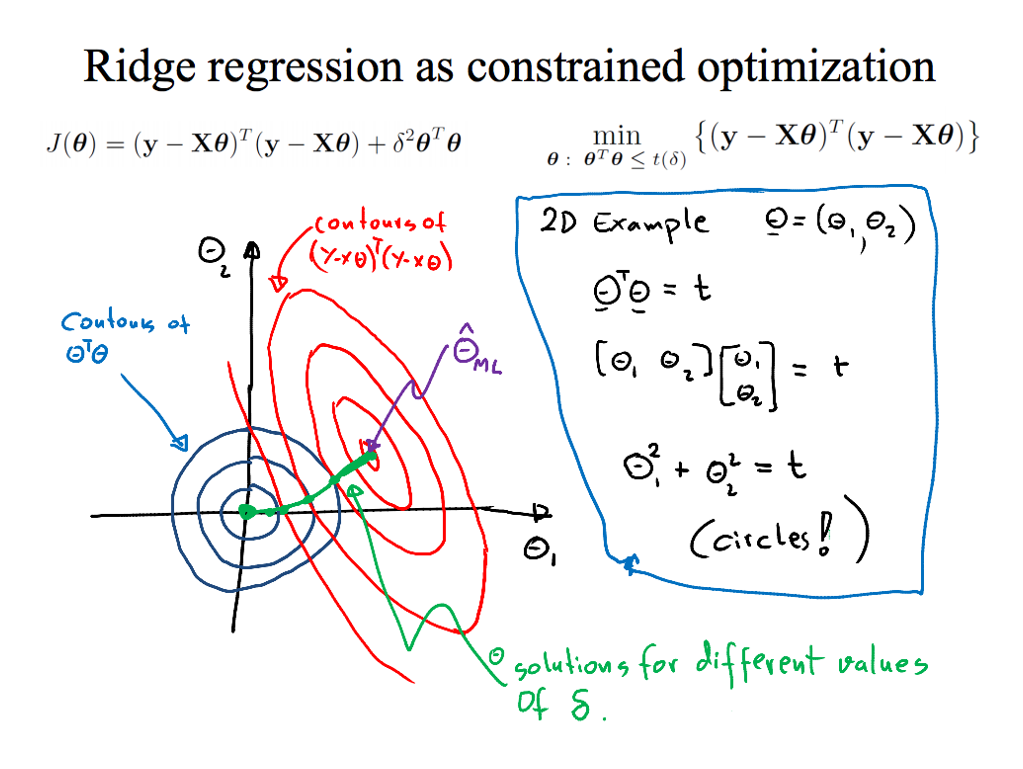
\includegraphics[width=0.5\textwidth]{Figures/regulation.eps}
    \caption{正则项的几何意义}
    \label{fig:1}
\end{figure*}




需要查找?? HIFT,JIST,HOG

\section{基础概念}
停止准则:与真值误差小于预设;两次迭代差小于预设;达到预设迭代次数

\section{分类}
\subsection{单层感知器}
单层感知器(Perception)解决线性可分问题,在高维空间用一个超平面划分样本。Rosenblatt证明两类模式线性可分时算法收敛。
\begin{equation}
\label{perception}
\begin{split}
&\boldsymbol Y = \sgn \left( [w_i,b] \dot [x_i,1]^T \right)=\sgn(\boldsymbol W^T \boldsymbol X)\\
&\boldsymbol W_{n+1}=\boldsymbol W_n + \eta (\boldsymbol Y_{\text{real} } -\boldsymbol Y_n ) \boldsymbol X_n 
\end{split}
\end{equation}
二值化,分类的边界距离某一类很接近。
常采用纠错学习规则的学习算法,把偏置作为固定输入
局限性:不能解决线性不可分问题。奇异样本训练时间长。只适合单层。



\end{document}